\section{Ejercicio 1: Control de bombas de agua}
Se pretende implementar un sistema controlador de dos bombas de agua cuya función es mantener el nivel de agua de un tanque entre un rango marcado por dos 
sensores de nivel.
Ambas bombas estarán encendidas cuando el nivel de agua esté por debajo del mínimo (sensor I=0), y apagadas cuando este supere el máximo (sensor S=1).
En un nivel intermedio (I=1 y S=0), solo una de las bombas se encontrará trabajando, y aquella en hacerlo será la última en haber permanecido apagada mientras la otra 
bomba estaba en funcionamiento; es decir, si en determinado momento está trabajando solo la bomba 1 (B1), la próxima vez que se dé la condición I=1 y S=0, se pondrá en 
funcionamiento la bomba 2 (B2), y vice versa.
Es en esta característica de \"memoria\" en donde el planteo de una solución a la problemática mediante una máquina de estados, se vuelve considerable.



\subsection{Diseño de Máquina de Estados}
Se propone como diseño para la máquina de estados aquella que sigue el diagrama de la Figura \ref{fig:fsm_state_chart_ex1}.
Cabe destacar que para la combinación de entradas I=0 y S=1, que resulta imposible en la aplicación del circuito a la realidad, dado que el sensor I se encuentra por 
debajo del sensor S, se decidió apagar ambas bombas por seguridad.
\begin{figure}[H]
    \centering
    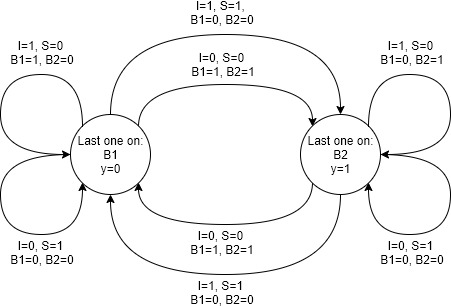
\includegraphics[width=0.7\textwidth]{../EJ1/Recursos/fsm_state_chart.jpg}
    \caption{Diagrama de estados para sistema de control de bombas.}
    \label{fig:fsm_state_chart_ex1}
\end{figure}

Como se puede observar, la máquina de estados planteada corresponde a una implementación de Mealy.
La decisión de utilizar esta implementación por sobre una de Moore, es que una aplicación estricta de la segunda, donde la salida dependiera únicamente del estado actual,
hubiera supuesto el uso de 6 estados, resultando altamente ineficiente en comparación a la solución elegida.\\
\\
La Tabla \ref{tab:truth_table_ex1} representa la tabla de verdad correspondiente a la máquina de estados en cuestión, donde \"y\" es el estado actual, \"I\" y \"S\" las entradas,
\"Y\" el siguiente estado a partir del próximo clock, y \"B1\" y \"B2\" las salidas asincrónicas. 
\begin{table}[H]
    \centering
    \begin{tabular}{ccc|ccc}
    \textbf{I} & \textbf{S} & \textbf{y} & Y & B1 & B2 \\ \hline
    0          & 0          & 0          & 1 & 1  & 1  \\
    0          & 0          & 1          & 0 & 1  & 1  \\
    0          & 1          & 0          & 0 & 0  & 0  \\
    0          & 1          & 1          & 1 & 0  & 0  \\
    1          & 0          & 0          & 0 & 1  & 0  \\
    1          & 0          & 1          & 1 & 0  & 1  \\
    1          & 1          & 0          & 1 & 0  & 0  \\
    1          & 1          & 1          & 0 & 0  & 0 
    \end{tabular}
    \caption{Tabla de verdad para máquina de estados de control de bombas.}
    \label{tab:truth_table_ex1}
    \end{table}

De la observación de las salidas, se infiere que los circuitos lógicos para implementarlas son los de las Figuras \ref{fig:Y_logic_circuit_ex5}, 
\ref{fig:B1_logic_circuit_ex5} y \ref{fig:B2_logic_circuit_ex5}.
Luego, la máquina de estados estará conformada por el circuito de la Figura \ref{fig:fsm_circtuit_ex5}.
\begin{figure}[H]
    \centering
    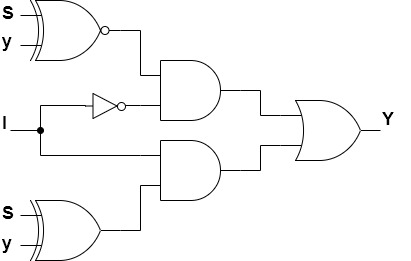
\includegraphics[width=0.4\textwidth]{../EJ1/Recursos/Y_logic_circuit.jpg}
    \caption{Circuito lógico para la entrada del Flip-Flop D.}
    \label{fig:Y_logic_circuit_ex5}
\end{figure}
\begin{figure}[H]
    \centering
    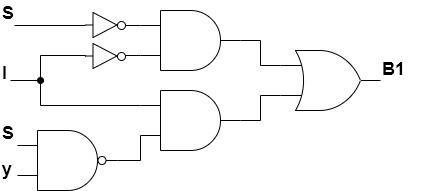
\includegraphics[width=0.4\textwidth]{../EJ1/Recursos/B1_logic_circuit.jpg}
    \caption{Circuito lógico para la salida de la bomba 1.}
    \label{fig:B1_logic_circuit_ex5}
\end{figure}
\begin{figure}[H]
    \centering
    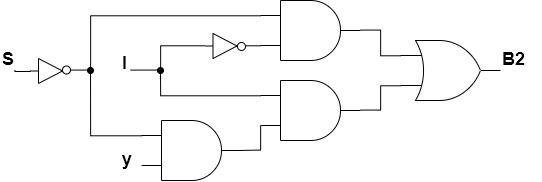
\includegraphics[width=0.4\textwidth]{../EJ1/Recursos/B2_logic_circuit.jpg}
    \caption{Circuito lógico para la salida de la bomba 2.}
    \label{fig:B2_logic_circuit_ex5}
\end{figure}
\begin{figure}[H]
    \centering
    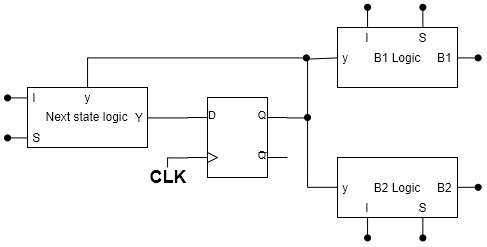
\includegraphics[width=0.7\textwidth]{../EJ1/Recursos/fsm_circuit.jpg}
    \caption{Circuito de la máquina de estados.}
    \label{fig:fsm_circtuit_ex5}
\end{figure}



\subsection{Simulaciones en Verilog}



\subsection{Diseño en PCB}



\subsection{Resultados}



\subsection{Conclusiones}